
\section{Results}

During the training phase of all the models proposed, we applied the cross-validation 
with $k=10$ groups to avoid overfit our models. We present as assessment metrics 
the ROC in Figure~\ref{fig:ROC}, except for both KNN models, since its model does not 
allows us to obtain the performance curve. We can conclude that non-linear methods, such as SVM and the Decision Trees with 100 nodes, have better performance when compared to simpler methods, such as Decision Trees with 10 nodes and Linear Methods.

However, this pattern does not hold on the test set, since the linear models obtained 
a quite good generalization capacity, making them as efficient as the non-linear models.

\begin{figure}[htbp!]
  \centerline{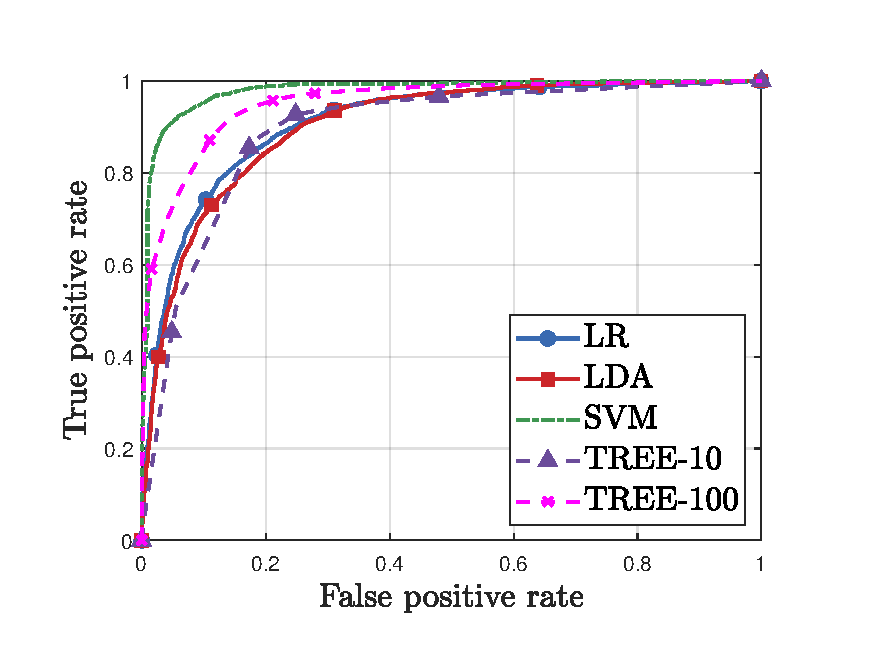
\includegraphics[width=0.5\textwidth]{../../code/hw3/matlab/figures/ROC.pdf}}
  \caption{ROC plot to illustrate the ability of each binary classifier system as its discrimination threshold is varied.}
  \label{fig:ROC}
\end{figure}

From the Table~\ref{tab:results}, we may assess the time necessary for train and test each model. SVM presents the best CV accurracy, howevere it presents the worst train duration, four times the second longest model train. The others methods present similar CV accuracy perfomance, while their cost is way less than SVM, except for KNN, with $K=1$. 
Among the presented methods, the test time is very short, less than a second.

The model choice depends on the scenario, the Decision Tree with ten nodes presents a very CV accuracy, similar to SVM, and it last less than a second to train. Hence, the advantages presented allow us to point out the decision tree as the best model.